\chapter{Design di dettaglio}\label{ch:design-di-dettaglio}
In seguito alla realizzazione del design architetturale di massima sono state effettuate scelte rilevanti
relative alla progettazione di alcune parti del sistema.

\section{Lista di componenti}\label{sec:lista-di-componenti}
Una caratteristica importante della libreria è permettere di specificare nel tipo di un sistema (o una view)
su quali componenti questi operano, così che le stesse firme dei metodi possano guidare il programmatore indicando i
tipi dei componenti trattati.
Così facendo si elimina la necessità di specificare a tempo di esecuzione il tipo di componenti richiesto (come per
esempio è necessario fare nella libreria Ashely~\cite{ashley} che ricorre al passaggio di oggetti \texttt{Class<?>})
permettendo d'intercettare diversi errori a tempo di compilazione.

Realizzare tale funzionalità a livello di compilazione si è rivelato essere una sfida che ha richiesto la definizione
delle \texttt{CList}, nonché l’utilizzo di macro per modificare il comportamento del compilatore introducendo controlli
personalizzati.

Una \texttt{CList} (abbreviazione di Components List) è essenzialmente una lista di elementi eterogenei che preserva
informazioni sul tipo di ciascun elemento in maniera simile a una tupla.
Per esempio si osservi il Listato~\ref{lst:lstinputlisting2}: la lista che contiene
i componenti \texttt{Position} e \texttt{Velocity} avrà come tipo~\texttt{Position~\&:~Velocity~\&:~CNil}, permettendo di conoscere il
tipo e la posizione dei suoi elementi.

Nel Listato~\ref{lst:lstinputlisting2} viene mostrato un esempio di utilizzo delle \texttt{CList} nelle~\texttt{View}.
\lstinputlisting[label={lst:lstinputlisting2}, caption=Esempio di utilizzo delle CList.]{code/clist-usage.scala}

L’idea alla base di questa soluzione è ispirata dalle \textit{Heterogeneous List} della libreria
Shapeless\cite{shapeless}; una differenza significativa sta nel fatto che la definizione di una \texttt{CList} impone un
limite ulteriore sul tipo dei suoi elementi: devono tutti essere sottotipi di \Component, parte dell’implementazione è
riportata al Listato~\ref{lst:lstinputlisting}.

\lstinputlisting[label={lst:lstinputlisting}, caption=Esempio di codice per implementare CList.]{code/clist.scala}

\section{Container di componenti}\label{sec:container-di-componenti}
Come è possibile osservare in Figura~\ref{fig:world-detail}, dal design di dettaglio emerge come
non siano le \Entity stesse a possedere i \Component che vengono loro assegnati.
Infatti, la gestione dei componenti è demandata ad un \texttt{ComponentsContainer}; questo permette
di aggiungere o rimuovere coppie entità-componente oppure di ottenere tutte le entità con uno specifico tipo
di componente.
In questo modo è possibile introdurre in maniera semplice ottimizzazioni nella gestione dei
componenti per rendere la loro iterazione (fondamentale per i \System) quanto più veloce possibile.

Grazie a questa scelta è stato piuttosto semplice modificare l'implementazione del
\texttt{ComponentsContainer} per attuare ottimizzazioni (descritte nel paragrafo~TODO)
necessarie a rispettare il requisito non funzionale~\ref{itm:nf1}.
\begin{figure}
    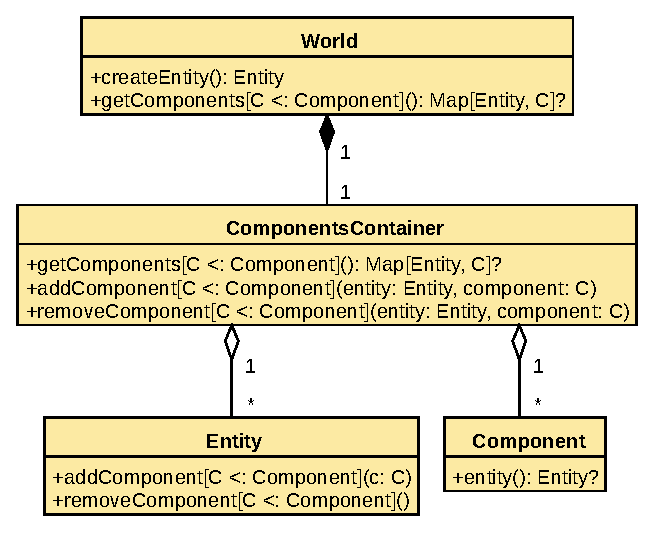
\includegraphics{./img/WorldDetail}
    \caption{Design di dettaglio di World e Entities}
    \label{fig:world-detail}
\end{figure}

\section{Builder dei sistemi}\label{sec:builder-dei-sistemi}
Si è scelto di realizzare il pattern \texttt{Builder} per permettere una creazione di \System
quanto più semplice possibile.
Come mostrato nel diagramma riportato in Figura~TODO il \texttt{SystemBuilder} dispone di diversi metodi per
specificare l'implementazione di alcuni dei metodi del sistema che verrà costruito.
Per completare la costruzione tramite il \texttt{Builder} e ottenere il nuovo sistema bisogna specificare
(tramite il metodo \texttt{withUpdate}) l'implementazione del suo metodo \texttt{update}.

\section{DSL}\label{sec:dsl}
